\chapter{实验系统介绍}{简介}

\section{性能概括}

嵌入式实验系统 x210v3 是基于 45 nm 工艺S5PV210芯片的开发平台。核心处理器
S5PV210 为 Cortex--A8架构, 主频可到 1GHz, 支持 1GiB DDR2, 片内32KiB I/D 缓存及
512KiB 二级缓存, PowerVR SGX540 图形加速引擎, 支持MPEG4、H.263、H.264 
1080P@30fps编码及MPEG4 1080P@30fps解码, HDMI/TV--OUT, 引脚间距 0.65mm, 
17$\times$17 mm FBGA封装。

x210v3 由核心板,底板和液晶板三大块组成,核心板采用 8 层板工艺设计,  底板留有
丰富的外设接口,几乎具备 210 所有功能的调试,液晶板采用 7英寸电容触摸屏。

\begin{figure}[!ht]
\centering
\includegraphics[width=.8\textwidth]{x210v3_board}
\caption{底板布局}
\end{figure}

\section{系统资源}

	系统硬件配置如下:

\begin{itemize}
  \item 内核:ARM Cortex-A8,主频 1GHz
  \item 内存:512MB
  \item Flash:4GB inand-Flash
  \item 24 位 RGB 接口
  \item 四路 USB HOST 接口
  \item USB OTG 接口
  \item 两路 RS232 接口
  \item SD 卡接口
  \item 四 LED 指示
  \item 功能按键(开机/复位等)
  \item HDMI高清视频接口
  \item 音频输入/输出接口
  \item 有线以太网 DM9000CEP;
  \item 电容触摸屏
  \item 摄像头接口
  \item 实时时钟
  \item 支持 G-sensor、 SPI、I2C、UART、USB/WiFi、GPS、GPRS等多种外围器件扩展
  \item MPEG2/MPEG4,H.263,H.264 视频编解码 1080P@30fps
  \item 2D/3D 高性能图形加速;
\end{itemize}

\section{软件}

在x210v3平台上, 可以进行 Linux、WinCE等多种操作系统的移植以及裸机实验。
本课程主要围绕 Linux 操作系统进行开发。

\subsection{交叉编译工具链 toolchain}
由于嵌入式系统的局限性,不可能具有很大的存储能力和友好的人机交互开发界面,
所以一般开发环境都必须安装在 PC 上,再通过 toolchain 生成最终目标文件,将其
运行在相应的目标平台上。

由于Cortex--A8 基于 ARM 体系结构, 所以在基于Cortex--A8 开发过程中
必须使用 ARM 的交叉编译。这个编译器环境将使用下面的 GNU 工具:
\begin{itemize}
  \item GNU gcc compilers for C, C++,包括编译器、链接器等;
  \item GNU binutil,包括归档、目标程序复制和转换、代码分析调试等工具;
  \item GNU C Library,支持目标代码的 C 语言库;
  \item GNU C header,头文件。
\end{itemize}
在 PC 上缺省安装的 GNU Tools 都是针对 x86 体系结构的,而上述的 GNU 交叉
编译工具是针对 ARM 的。最终编译后产生的二进制文件只能在 ARM 架构的处理器上
运行。

\subsection{工具链安装}
GNU 工具链提供完整的源代码,可以在 PC 机上用x86 平台的编译工具编译安装,
也可以直接下载二进制代码包解压安装。
许多 Linux 的发行版软件仓库中已包含了 ARM 的交叉编译工具,可以考虑直接
使用。

本实验使用的交叉编译工具链路径是 /usr/local/arm-2009q3, 可执行程序在
 /usr/local/arm-2009q3/bin 目录下。 实验中请将该目录添加到环境变量 ``PATH''
中, 或给出完整的路径和编译程序名, 如
/usr/local/arm-2009q3/bin/arm-none-linux-gnueabi-gcc

\subsection{嵌入式系统软件}
嵌入式操作系统软件从下到上通常由 BootLoader、操作系统、文件系统和应用软件
等若干层构成,各层之间没有必然的依赖关系。可以用U-Boot-v2016.11-rc3 引导
Linux-4.9.19,也可以用 U-Boot-v2017-09-rc2 引导 Linux-3.0.8;在 Linux-3.0.8
版本上可以运行 glibc-2.10.1,也可以运行 glibc-2.23。依赖关系多出现在
具体功能上,例如在 Linux-3.0.8 的内核中找不到某个设备的驱动,而在稍后的
某个版本中该驱动才加入内核主线。

BootLoader的目的是加载并引导操作系统运行,有时也会负责文件系统
的加载。BootLoader还负责核心软件的升级。一旦操作系统启动, BootLoader 的任务
便暂告终结,直到系统重启。

本系统使用的bootloader名为u-boot。根据本实验系统特点, 厂家对u-boot做了
针对性的修改, 例如对inand-Flash操作以及支持Android系统升级的 fastboot 模式。

厂家在此平台上移植的 Linux 操作系统内核版本是2.6.35 和 3.0.8 (移植
Android 4.0.4使用的内核版本是3.0.8)。用户可在此基础上进一步剪裁和优化。
完成内核正常启动后,
与硬件相关的工作基本上都可以由内核解决, 以后的软件开发可以由用户自由发挥,
例如移植不同版本的根文件系统、不同的图形用户接口、桌面等。
